\documentclass[]{article}
\usepackage{amsmath}
\usepackage{amsfonts}
\usepackage{amssymb}
\usepackage{algorithmic}
\usepackage{algorithm}
\usepackage{tikz}
\usepackage{graphicx}
\usepackage{mdframed}
\usepackage{paralist}
\usepackage{listings}

\definecolor{dkgreen}{rgb}{0,0.6,0}
\definecolor{gray}{rgb}{0.5,0.5,0.5}

\lstset{
  language=Python,
  breaklines=true,
  showstringspaces=false,
  frame=single,
  aboveskip=3mm,
  belowskip=3mm,
  columns=flexible,
  basicstyle={\small\ttfamily},
  numbers=none,
  numberstyle=\tiny\color{gray},
  keywordstyle=\color{blue},
  commentstyle=\color{gray},
  stringstyle=\color{dkgreen},
  breakatwhitespace=true,
  tabsize=3
}

\title{CAGD - Homework 5}
\author{Josefine St{\aa}l \& Erik Ackzell}

\begin{document}

\maketitle

\section*{Task 1}
In this task we convert between barycentric and homogeneous coordinates.\\
Consider the points \begin{equation*}
p_0 = \left(\begin{array}{c}
1\\
1\\
1
\end{array}\right), \quad
p_1 = \left(\begin{array}{c}
3\\
3\\
3
\end{array}\right), \quad
p_2 = \left(\begin{array}{c}
1\\
2\\
2
\end{array}\right)
\end{equation*}
and let \begin{equation*}
q_1=\left(\begin{array}{c}
0.25\\
0.25\\
0.5
\end{array}\right)
\end{equation*}
in barycentric coordinates with respect to $p_0, p_1, p_2$. We want to express $q_1$ in homogeneous coordinates.\\
First, we express $q_1$ in Cartesian coordinates \begin{equation*}
q_1 = 0.25p_0 + 0.25p_1 + 0.5p_2 = \left(\begin{array}{c}
0.25 + 1.5 + 0.25\\
0.25 + 1.5 + 0.5\\
0.25 + 1.5 + 0.5
\end{array}\right) = \left(\begin{array}{c}
2\\
2.25\\
2.25
\end{array}\right).
\end{equation*}
For any $\omega\in\mathbb{R}$, the homogeneous coordinates of $q_1$ are\begin{equation*}
q_1 = \left(\begin{array}{c}
2\omega\\
2.25\omega\\
2.25\omega\\
\omega
\end{array}\right),
\end{equation*}
which is what we wanted to determine.\\
Now let \begin{equation*}
q_2 = \left(\begin{array}{c}
5\\
4\\
4\\
3
\end{array}\right)
\end{equation*}
in homogeneous coordinates. We wish to express $q_2$ in barycentric coordinates with respect to $p_0, p_1, p_2$.\\
First, we express $q_2$ in Cartesian coordinates \begin{equation*}
q_2 = \frac{1}{3}\left(\begin{array}{c}
5\\
4\\
4
\end{array}\right).
\end{equation*}
We now want to determine the coefficients $a_0, a_1, a_2$ such that \begin{equation*}
\sum_{i=0}^{2}a_ip_i
\end{equation*}
and \begin{equation*}
\sum_{i=0}^{2}a_i=1.
\end{equation*}
This can be done by solving the linear equation system \begin{equation*}
\left(\begin{array}{ccc}
1 & 3 & 1\\
1 & 3 & 2\\
1 & 3 & 2\\
1 & 1 & 1
\end{array}\right)\left(\begin{array}{c}
a_0\\
a_1\\
a_2
\end{array}\right) = \frac{1}{3}\left(\begin{array}{c}
5\\
4\\
4\\
3
\end{array}\right),
\end{equation*}
which reduces to \begin{equation*}
\left(\begin{array}{ccc}
1 & 3 & 1\\
1 & 3 & 2\\
1 & 1 & 1
\end{array}\right)\left(\begin{array}{c}
a_0\\
a_1\\
a_2
\end{array}\right) = \frac{1}{3}\left(\begin{array}{c}
5\\
4\\
3
\end{array}\right).
\end{equation*}
The solution is given by \begin{equation*}
a_0 = 1, \quad a_1 = \frac{1}{3}, \quad a_2 = -\frac{1}{3},
\end{equation*}
so in barycentric coordinates with respect to $p_0, p_1, p_2$, \begin{equation*}
q_2 = \frac{1}{3}\left(\begin{array}{r}
3\\
1\\
-1
\end{array}\right),
\end{equation*}
which is what we wanted to determine.
%\begin{figure}[h!]
%	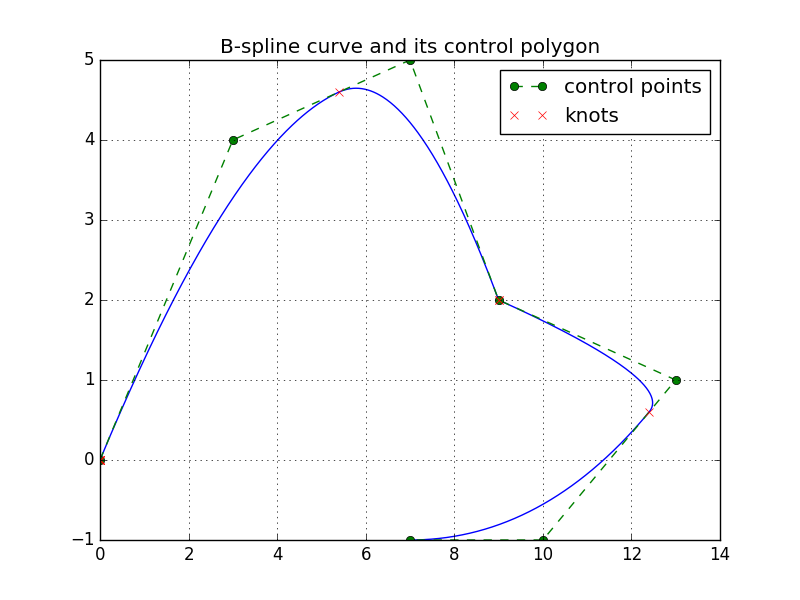
\includegraphics[scale=0.6]{bspline}
%\end{figure}

\section*{Do-over Homework 2 Task 5}
In this task we want to determine whether the Lagrange and monomial forms are invariant under affine 	domain transformations. We show that the Lagrange form is \textbf{not} invariant under all domain transformations and that the monomial form is invariant under domain transformations.\\
\\
\textbf{Claim:} The Lagrange form is not invariant under all domain transformations.\\
\textbf{Proof:} Assume that the Lagrange form is invariant under all domain transformation, and define the domain transformation \begin{equation*}
\varphi: [-3, 3] \rightarrow [0, 1]
\end{equation*}
by
\begin{equation*}
\varphi(x) = \frac{x + 3}{6}.
\end{equation*}
We know that the Lagrange basis polynomial of degree $n$ is on the form\begin{equation*}
L_i^n(x) = \prod_{j=0, j\neq i}^{n}\frac{x-x_i}{x_i - x_j}
\end{equation*}
And that any polynomial \begin{equation*}
p:[-3, 3]\rightarrow \mathbb{R}
\end{equation*}
of degree $n$ can be expressed as \begin{equation*}
p(x)=\sum_{i = 0}^{n} c_iL_i^n(x).
\end{equation*}
Set $n=1$, $c_0 = 2$, $c_1 = 3$, $x_0=-3$ and $x_1 = 3$ and define \begin{equation*}
p(x)=\sum_{i = 0}^{1} c_iL_i^1(x).
\end{equation*}
We have that, for $x=1$ \begin{equation*}
\begin{aligned}
\varphi(p(1)) &= \varphi\left(\sum_{i = 0}^{1}c_iL_i^1(1)\right)\\
&=\varphi\left(c_0L_0^1(1) + c_1L_1^1(1)\right)\\
&=\varphi\left(- 2 \cdot\frac{4}{6} - 3\cdot\frac{2}{6}\right)\\
&=\varphi\left(- \frac{8}{6} - \frac{6}{6}\right)\\
&=\varphi\left(-\frac{7}{3}\right)\\
&=-\frac{7}{18} + \frac{1}{2}\\
&=\frac{2}{9}.
\end{aligned}
\end{equation*}
Furthermore, we have that \begin{equation*}
\begin{aligned}
\sum_{i = 0}^{1}\varphi(c_i)L_i^1(1) &= -\varphi(c_0)\cdot \frac{2}{3} - \varphi(c_1)\cdot\frac{1}{3}\\
&=-\frac{5}{6}\cdot\frac{2}{3} - 1 \cdot \frac{1}{3}\\
&=-\frac{10}{18} - \frac{6}{18}\\
&=-\frac{8}{9}.
\end{aligned}
\end{equation*}

\newpage
\section*{Appendix I}
%\lstinputlisting[lastline=87]{bsplines.py}

\end{document}
